\documentclass[12pt]{article}
\usepackage[left=15mm,top=0.5in,bottom=0.5in,centering]{geometry}
\usepackage{listings}
\usepackage{framed}
\usepackage{graphicx}
\usepackage{wrapfig}
\usepackage{floatrow}
\usepackage{subfigure}
\usepackage{color}
\usepackage{amsmath}
\usepackage{lipsum}
\usepackage{hyperref}
\usepackage{amssymb}
\usepackage{rotating}
\usepackage{tikz}
\usepackage{tabu}
\usepackage{titlesec}
%\usepackage{algorithm}
\usepackage[linesnumbered,ruled,vlined,english,onelanguage]{algorithm2e}
%\usepackage{algorithmic}
\usepackage[noend]{algpseudocode}
\definecolor{dkgreen}{rgb}{0,0.6,0}
\definecolor{gray}{rgb}{0.5,0.5,0.5}
\definecolor{mauve}{rgb}{0.58,0,0.82}
\lstset{frame=tb,
	language=Java,
	aboveskip=3mm,
	belowskip=3mm,
	showstringspaces=false,
	columns=flexible,
	basicstyle={\small\ttfamily},
	numbers=none,
	numberstyle=\tiny\color{gray},
	keywordstyle=\color{blue},
	commentstyle=\color{dkgreen},
	stringstyle=\color{mauve},
	breaklines=true,
	breakatwhitespace=true,
	tabsize=3
}
\newcounter{question}
\setcounter{question}{0}
\def\thequestion{{\bf{Question \arabic{question}. }}\space }
\newcommand{\Question}[1]{\pagebreak \stepcounter{question}\noindent\thequestion#1\par}
\newcounter{countpart}[question]
\setcounter{countpart}{0}
\def\thepart{\\ \par (\alph{countpart}) \space}
\newcommand{\Part}[1]{\stepcounter{countpart}\noindent\thepart#1\normalfont{}}
\newenvironment{Parts}{\par\medskip
	\noindent \rmfamily}{\medskip}

\def\BeginSolution{\begin{framed}\noindent \normalfont{}}
	\def\EndSolution{\end{framed}\pagebreak}
\newcommand{\mat}[1]{\mathbf{#1}}
\newcommand{\matG}[1]{\boldsymbol{#1}}
\newcommand{\bm}[1]{\boldsymbol{#1}}
\def\real{\mathbb{R}}
\def\R{\mathbb{R}}
\newcommand{\norm}[1]{\left\lVert#1\right\rVert}
%\newcommand*\EE[1]{\ensuremath{\text{\textsc{e}}#1}}
\def\EE{\mathbb{E}}
\def\ev{\mathbb{E}}
\def\P{\mathbf{P}}
\def\y{\vec{y}}
\def\X{\mathbf{X}}
\def\x{\vec{x}}
\def\w{\vec{w}}
\def\b{\vec{b}}
\def\r{\vec{r}}
\def\T{^{\top}}
\def\argmin{\text{arg}\min\limits}
\def\argmax{\text{arg}\max\limits}
\def\I{\mathbb{I}}
\def\A{\vec{A}}
\def\tran{^{\top}}
\def\W{\mathbf{W}}
\def\z{\mathbb{z}}
\def\ell{l}
\newcommand{\diag}{\mathop{\mathrm{diag}}}
\allowdisplaybreaks
\usepackage[final]{pdfpages}
\setboolean{@twoside}{false}
\setcounter{MaxMatrixCols}{20}
%\usepackage[showframe]{geometry}

\usepackage{titling}
\renewcommand\maketitlehooka{\null\mbox{}\vfill}
\renewcommand\maketitlehookd{\vfill\null}

\title{CS294-112 HW2\vspace{-2ex}}
\author{Huanjie Sheng, 25928718\vspace{-2ex}}
\date{\today \vspace{-2ex}}

\begin{document}
	
	%\begin{titlingpage}
	%	\maketitle
	%\end{titlingpage}
	%\addcontentsline{toc}{subsection}{Appendices}
	\renewcommand{\thesubsection}{(\alph{subsection})}
	\renewcommand{\thesection}{Problem \arabic{section}.}
	\newcommand{\sectionbreak}{\clearpage}
	%\titleformat*{\subsection}{\normalfont}
	
	%\stepcounter{subsection}
	\section{State-dependent baseline}
	\subsection{Use linearity of expectation} 
	Here we want to show that
	\begin{align*}
		\mathbb{E}_{(\tau)\sim p_\theta(\tau)}\left[\sum_{t=1}^{T} \nabla_\theta \log \pi_\theta(a_t|s_t) b(s_t)\right] = 0
	\end{align*}
	We use the definition of expectation and expand the LHS before pushing the gradient into the summation and integral:
	\begin{align*}
	  & \mathbb{E}_{(\tau)\sim p_\theta(\tau)}\left[\sum_{t=1}^{T} \nabla_\theta \log \pi_\theta(a_t|s_t) b(s_t)\right] \\
	= & \sum_{t=1}^{T} \mathbb{E}_{(\tau)\sim p_\theta(\tau)}\left[ \nabla_\theta \log \pi_\theta(a_t|s_t) b(s_t)\right] \\
	= & \sum_{t=1}^{T} \int_\tau \nabla_\theta \log \pi_\theta(a_t|s_t) b(s_t) p_\theta(\tau) d_{\tau} \\
	= & \sum_{t=1}^{T} \int_{(s_t, a_t)} \int_{\tau/s_t, a_t|s_t, a_t} \nabla_\theta \log \pi_\theta(a_t|s_t) b(s_t) p_\theta(s_t, a_t)p_\theta(\tau/s_t, a_t|s_t, a_t) d_{\tau/s_t, a_t} d_{(s_t, a_t)} \\
	= & \sum_{t=1}^{T} \int_{(s_t, a_t)}  \left[\int_{\tau/s_t, a_t|s_t, a_t} p_\theta(\tau/s_t, a_t|s_t, a_t) d_{\tau/s_t, a_t} \right] \nabla_\theta \log \pi_\theta(a_t|s_t) b(s_t) p_\theta(s_t, a_t) d_{(s_t, a_t)}  \\
	= & \sum_{t=1}^{T} \int_{(s_t, a_t)}  \nabla_\theta \log \pi_\theta(a_t|s_t) b(s_t) p_\theta(s_t, a_t) d_{(s_t, a_t)}  \\
	= & \sum_{t=1}^{T} \int_{s_t} \int_{a_t} \nabla_\theta \log \pi_\theta(a_t|s_t) b(s_t) p_\theta(s_t) \pi_\theta(a_t|s_t) d_{a_t} d_{s_t}  \\
	= & \sum_{t=1}^{T} \int_{s_t} \left[\int_{a_t}  \pi_\theta(a_t|s_t) \nabla_\theta \log \pi_\theta(a_t|s_t) d_{a_t} \right] b(s_t) p_\theta(s_t)   d_{s_t}  \\
	= & \sum_{t=1}^{T} \int_{s_t} \left[\int_{a_t}  \nabla_\theta \pi_\theta(a_t|s_t) d_{a_t} \right] b(s_t) p_\theta(s_t)   d_{s_t}  \\
	= & \sum_{t=1}^{T} \int_{s_t} \left[\nabla_\theta \int_{a_t}  \pi_\theta(a_t|s_t) d_{a_t} \right] b(s_t) p_\theta(s_t)   d_{s_t}  \\
	= & \sum_{t=1}^{T} \int_{s_t} \left[\nabla_\theta 1 \right] b(s_t) p_\theta(s_t)   d_{s_t}  \\
	= & \sum_{t=1}^{T} \int_{s_t} \left[0 \right] b(s_t) p_\theta(s_t)   d_{s_t}  \\
	= & 0
	\end{align*}
	\pagebreak
	\subsection{An alternative approach}
	(a) Because we assume Markov properties for our Markov decision process, the state transition probability $p(s_{t^*+1}|s_{t^*}, a_{t^*})$ and the policy $\pi(a_{t^*}|s_{t^*})$ only depend on current state not the history.  Besides, $b(s_{t^*})$ only depends on state but not the action.  Therefore, for the inner expectation, conditioning on $(s_1, a_1, \dots, a_{t^*-1}, s_{t^*})$ is equivalent to conditioning only on $s_{t^*}$. \\
	(b) For ease of notation, I denote $(s_1, a_1, \dots, a_{t^*-1}, s_{t^*})$ as $(s_{1:t^*}, a_{1:t^*-1})$. 
	\begin{align*}
	& \mathbb{E}_{(\tau)\sim p_\theta(\tau)}\left[\sum_{t=1}^{T} \nabla_\theta \log \pi_\theta(a_t|s_t) b(s_t)\right] \\
	= & \sum_{t=1}^{T} \mathbb{E}_{(\tau)\sim p_\theta(\tau)}\left[ \nabla_\theta \log \pi_\theta(a_t|s_t) b(s_t)\right] \\
	= & \sum_{t=1}^{T} \int_\tau \nabla_\theta \log \pi_\theta(a_t|s_t) b(s_t) p_\theta(\tau) d_{\tau} \\
	= & \sum_{t=1}^{T} \int \int \nabla_\theta \log \pi_\theta(a_t|s_t) b(s_t) p_\theta(s_{1:t}, a_{1:t-1})p_\theta(s_{t+1:T}, a_{t:T}|s_{1:t}, a_{1:t-1}) d_{(s_{t+1:T}, a_{t:T}|s_{1:t}, a_{1:t-1})} d_{(s_{1:t}, a_{1:t-1})} \\
	= & \sum_{t=1}^{T} \int \int \nabla_\theta \log \pi_\theta(a_t|s_t) b(s_t) p_\theta(s_{1:t}, a_{1:t-1})p_\theta(s_{t+1:T}, a_{t:T}|s_t) d_{(s_{t+1:T}, a_{t:T}|s_t)} d_{(s_{1:t}, a_{1:t-1})} \\
	= & \sum_{t=1}^{T} \int \left[\int \nabla_\theta \log \pi_\theta(a_t|s_t) p_\theta(s_{t+1:T}, a_{t:T}|s_t) d_{(s_{t+1:T}, a_{t:T}|s_t)} \right]  b(s_t) p_\theta(s_{1:t}, a_{1:t-1}) d_{(s_{1:t}, a_{1:t-1})} \\
	= & \sum_{t=1}^{T} \int \left[\int \int_{a_t} \pi_\theta(a_t|s_t) \nabla_\theta \log \pi_\theta(a_t|s_t) p_\theta(s_{t+1:T}, a_{t+1:T}|s_t) d_{a_t} d_{(s_{t+1:T}, a_{t+1:T}|s_t)} \right]  b(s_t) p_\theta(s_{1:t}, a_{1:t-1}) d_{(s_{1:t}, a_{1:t-1})} \\
	= & \sum_{t=1}^{T} \int \int \left[\int_{a_t} \pi_\theta(a_t|s_t) \nabla_\theta \log \pi_\theta(a_t|s_t) d_{a_t} \right] p_\theta(s_{t+1:T}, a_{t+1:T}|s_t) d_{(s_{t+1:T}, a_{t+1:T}|s_t)}   b(s_t) p_\theta(s_{1:t}, a_{1:t-1}) d_{(s_{1:t}, a_{1:t-1})} \\
	= & \sum_{t=1}^{T} \int \int \left[\int_{a_t} \nabla_\theta  \pi_\theta(a_t|s_t) d_{a_t} \right] p_\theta(s_{t+1:T}, a_{t+1:T}|s_t) d_{(s_{t+1:T}, a_{t+1:T}|s_t)}   b(s_t) p_\theta(s_{1:t}, a_{1:t-1}) d_{(s_{1:t}, a_{1:t-1})} \\
	= & \sum_{t=1}^{T} \int \int \left[ \nabla_\theta  \int_{a_t} \pi_\theta(a_t|s_t) d_{a_t} \right] p_\theta(s_{t+1:T}, a_{t+1:T}|s_t) d_{(s_{t+1:T}, a_{t+1:T}|s_t)}   b(s_t) p_\theta(s_{1:t}, a_{1:t-1}) d_{(s_{1:t}, a_{1:t-1})} \\
	= & \sum_{t=1}^{T} \int \int \left[ \nabla_\theta  1 \right] p_\theta(s_{t+1:T}, a_{t+1:T}|s_t) d_{(s_{t+1:T}, a_{t+1:T}|s_t)}   b(s_t) p_\theta(s_{1:t}, a_{1:t-1}) d_{(s_{1:t}, a_{1:t-1})} \\
	= & \sum_{t=1}^{T} \int \int \left[ 0 \right] p_\theta(s_{t+1:T}, a_{t+1:T}|s_t) d_{(s_{t+1:T}, a_{t+1:T}|s_t)}   b(s_t) p_\theta(s_{1:t}, a_{1:t-1}) d_{(s_{1:t}, a_{1:t-1})} \\
	= & 0
	\end{align*}
	
	\stepcounter{section}
	\stepcounter{section}
	\section{CartPole}
	
	\subsection{Figure}
	
	\begin{figure}[!htbp]
		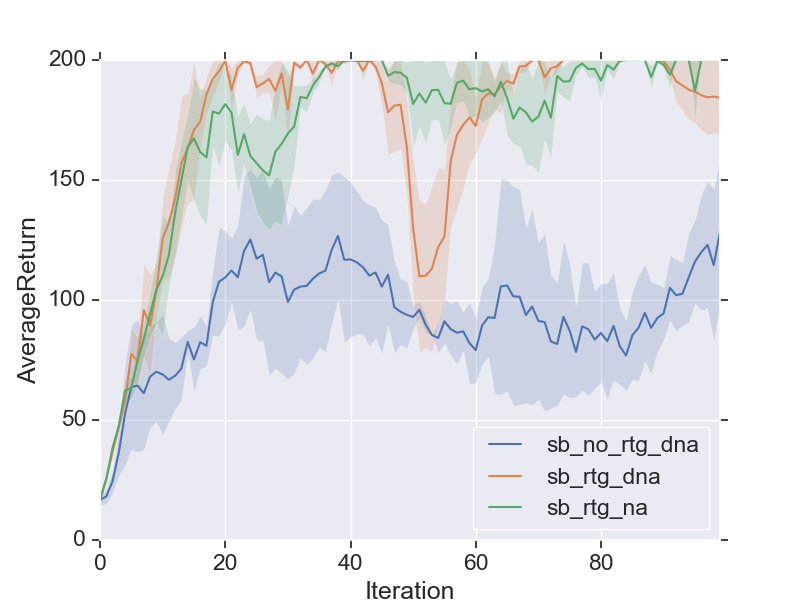
\includegraphics[width=0.48\textwidth]{problem4a.png}
		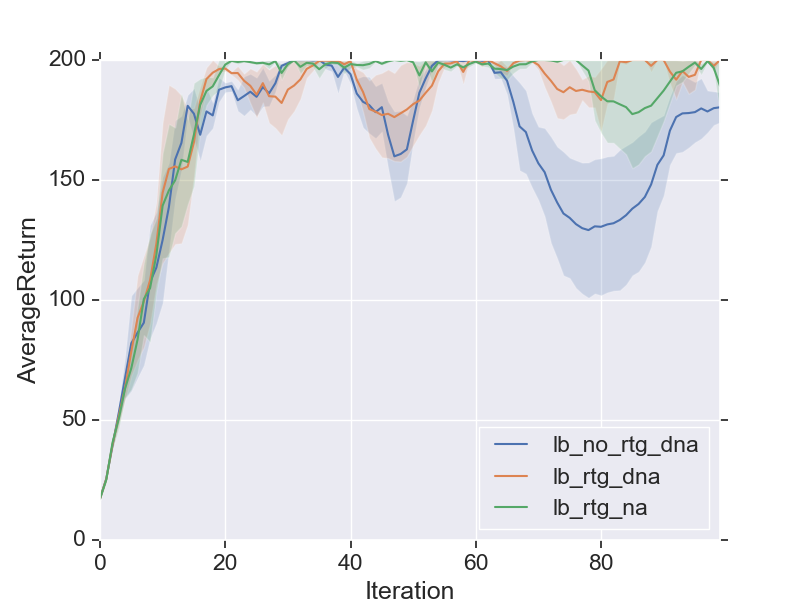
\includegraphics[width=0.48\textwidth]{problem4b.png}
	\end{figure}

	\subsection{Questions}

	\texttt{Which gradient estimator has better performance without advantage-centering the trajectory-centric one, or the one using reward-to-go?}\\
	In the small batch size case, the one using reward-to-go is better.  This is because it has low variance and smaller number so it's easier for NN to fit.\\
	In the large batch size case, they are all similar.\\
	\hfill \linebreak
	\texttt{Did advantage centering help?}\\
	It helps to stabilize the result as we can see that without centering the learning curve drops a little bit in the middle on the small batch size plot.\\
	In the large batch size case, they are all similar.\\
	
	\hfill \linebreak
	\texttt{Did the batch size make an impact?}\\
	Yes. Large batch size makes all curves similar this is because more data can help for NN to fit and it can reduce variance for each gradient step. Small batch size requires more careful manipulation to reduce variance.
	
	\subsection{Commands}
	\begin{minipage}{\linewidth}
		\begin{lstlisting}
		# Problem 4:
		
		# For small batch size simulation:
		
		python train_pg_f18.py CartPole-v0 -n 100 -b 1000 -e 3 -dna --exp_name sb_no_rtg_dna
		python train_pg_f18.py CartPole-v0 -n 100 -b 1000 -e 3 -rtg -dna --exp_name sb_rtg_dna
		python train_pg_f18.py CartPole-v0 -n 100 -b 1000 -e 3 -rtg --exp_name sb_rtg_na
		
		# For small batch size plot:
		
		python plot.py data/sb_no_rtg_dna_CartPole-v0_16-09-2018_16-29-21 data/sb_rtg_dna_CartPole-v0_16-09-2018_16-39-41 data/sb_rtg_na_CartPole-v0_16-09-2018_16-44-01 --value AverageReturn
		
		# For large batch size simulation:
		
		python train_pg_f18.py CartPole-v0 -n 100 -b 5000 -e 3 -dna --exp_name lb_no_rtg_dna
		python train_pg_f18.py CartPole-v0 -n 100 -b 5000 -e 3 -rtg -dna --exp_name lb_rtg_dna
		python train_pg_f18.py CartPole-v0 -n 100 -b 5000 -e 3 -rtg --exp_name lb_rtg_na
		
		# For large batch size plot:
		
		python plot.py data/lb_no_rtg_dna_CartPole-v0_16-09-2018_18-52-20 data/lb_rtg_dna_CartPole-v0_16-09-2018_18-54-25 data/lb_rtg_na_CartPole-v0_16-09-2018_18-56-55 --value AverageReturn
		\end{lstlisting}
	\end{minipage}
	
	\pagebreak
	
	\section{InvertedPendulum}
	\subsection{Figure}
	max\_score:1000.0, batch\_size:10000, learning\_rate:0.01
	\begin{figure}[!htbp]
		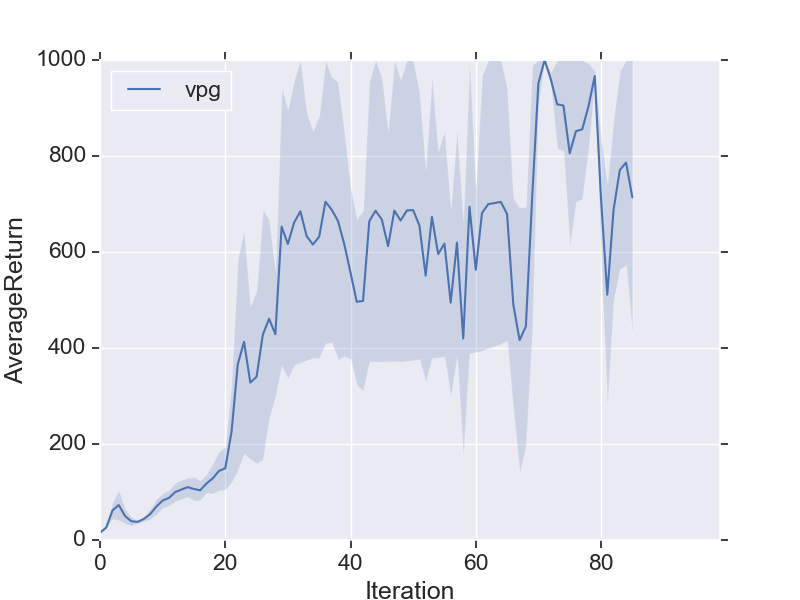
\includegraphics[width=0.5\textwidth]{problem5.png}
	\end{figure}

	\begin{minipage}{\linewidth}
	\begin{lstlisting}
	# Problem 5: 
	# 1. comment out main() and uncomment prob5()
	# 2. run the following command:
	
	python train_pg_f18.py InvertedPendulum-v2 -ep 1000 --discount 0.9 -n 100 -e 3 -l 2 -s 64 -rtg
	
	# 3. record the best batch size and learning rate:
	# max_score:1000.0, batch_size:10000, learning_rate:0.01
	
	# To answer the question, use the following commands:
	
	python train_pg_f18.py InvertedPendulum-v2 -ep 1000 --discount 0.9 -n 100 -e 3 -l 2 -s 64 -rtg -lr 0.01 -b 10000
	python plot.py data/vpg_InvertedPendulum-v2_16-09-2018_17-32-43 --value AverageReturn
	\end{lstlisting}
	\end{minipage}
	
	
	\stepcounter{section}
	\section{LunarLander}
	\subsection{Figure}
	\begin{figure}[!htbp]
		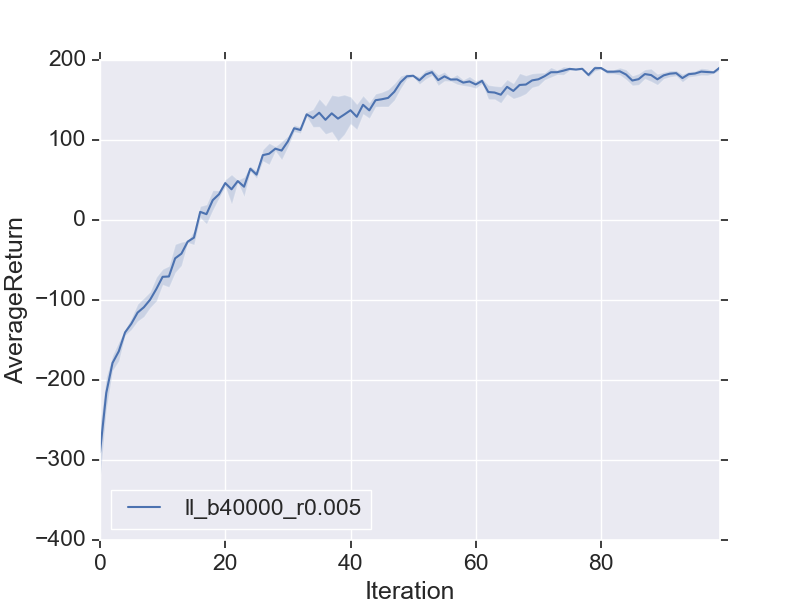
\includegraphics[width=0.5\textwidth]{problem7.png}
	\end{figure}
	\begin{minipage}{\linewidth}
	\begin{lstlisting}
	# Problem 7.
	python train_pg_f18.py LunarLanderContinuous-v2 -ep 1000 --discount 0.99 -n 100 -e 3 -l 2 -s 64 -b 40000 -lr 0.005 -rtg --nn_baseline --exp_name ll_b40000_r0.005
	
	python plot.py data\ll_b40000_r0.005_LunarLanderContinuous-v2_16-09-2018_17-40-36
	\end{lstlisting}
	\end{minipage}
	
	\section{HalfCheetah}
	\subsection{Question}
	\texttt{How did the batch size and learning rate affect the performance?}\\
	Large batch size increases the performance because we have more data to estimate the gradient. Small learning rate is bad because it converges slowly. It's shown on the left panel.\\
	\begin{figure}[h!]
		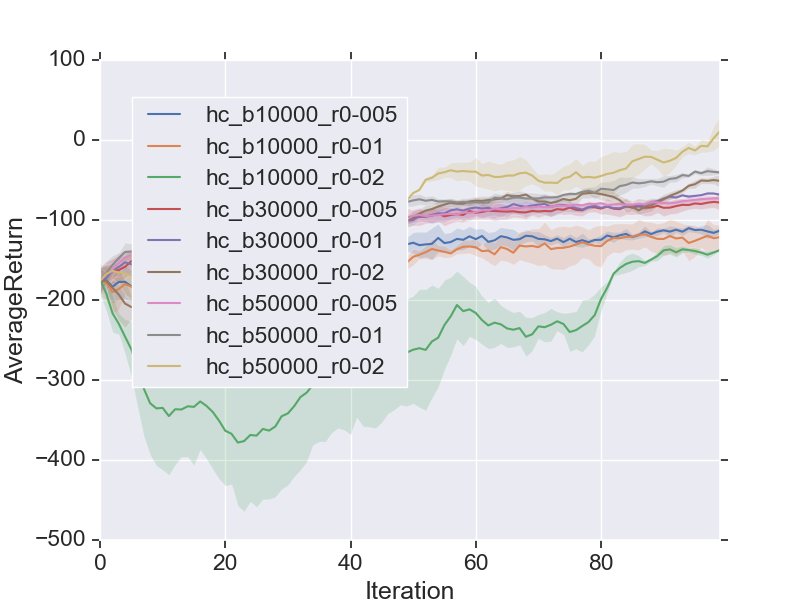
\includegraphics[width=0.48\textwidth]{problem8a.png}
		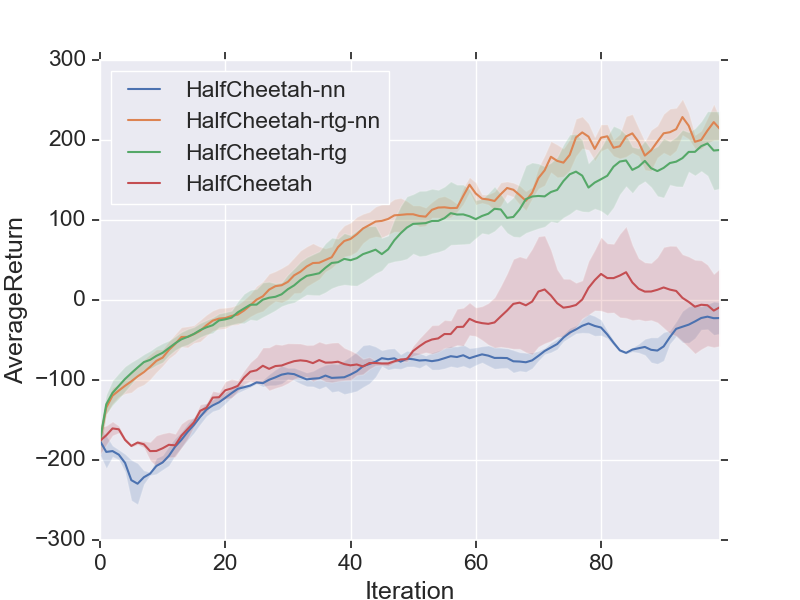
\includegraphics[width=0.48\textwidth]{problem8b.png}
	\end{figure}
	\\
	\begin{minipage}{\linewidth}
	\begin{lstlisting}
	# Problem 8:
	# 0. In get_log_prob(), I switched to MultivariateNormalDiag at this point
	# 1. comment out main() and uncomment prob8()
	# 2. run the following command:
	
	python train_pg_f18.py HalfCheetah-v2 -ep 150 --discount 0.95 -n 100 -e 3 -l 2 -s 32 -rtg --nn_baseline
	
	# 3. record the best batch size and learning rate:
	# max_score:10., batch_size:50000, learning rate:0.01
	
	python train_pg_f18.py HalfCheetah-v2 -ep 150 --discount 0.95 -n 100 -e 3 -l 2 -s 32 -b 50000 -lr 0.02 --exp_name HalfCheetah
	python train_pg_f18.py HalfCheetah-v2 -ep 150 --discount 0.95 -n 100 -e 3 -l 2 -s 32 -b 50000 -lr 0.02 -rtg --exp_name HalfCheetah-rtg
	python train_pg_f18.py HalfCheetah-v2 -ep 150 --discount 0.95 -n 100 -e 3 -l 2 -s 32 -b 50000 -lr 0.02 --nn_baseline --exp_name HalfCheetah-nn
	python train_pg_f18.py HalfCheetah-v2 -ep 150 --discount 0.95 -n 100 -e 3 -l 2 -s 32 -b 50000 -lr 0.02 -rtg --nn_baseline --exp_name HalfCheetah-rtg-nn
	
	python plot.py data/HalfCheetah-nn_HalfCheetah-v2_18-09-2018_00-50-50 data\HalfCheetah-rtg-nn_HalfCheetah-v2_18-09-2018_10-43-21 data\HalfCheetah-rtg_HalfCheetah-v2_18-09-2018_00-19-41 data\HalfCheetah_HalfCheetah-v2_17-09-2018_23-52-16
	\end{lstlisting}
	\end{minipage}
	
	\section*{Bonus}
	
	\par\itshape
	In PG, we collect a batch of data, estimate a single gradient, and then discard the data and move on. Can we potentially accelerate PG by taking multiple gradient descent steps with the same batch of data? Explore this option and report on your results. Set up a fair comparison between single-step PG and multi-step PG on at least one MuJoCo gym environment.
	\par
	
	\begin{figure}[!htbp]
		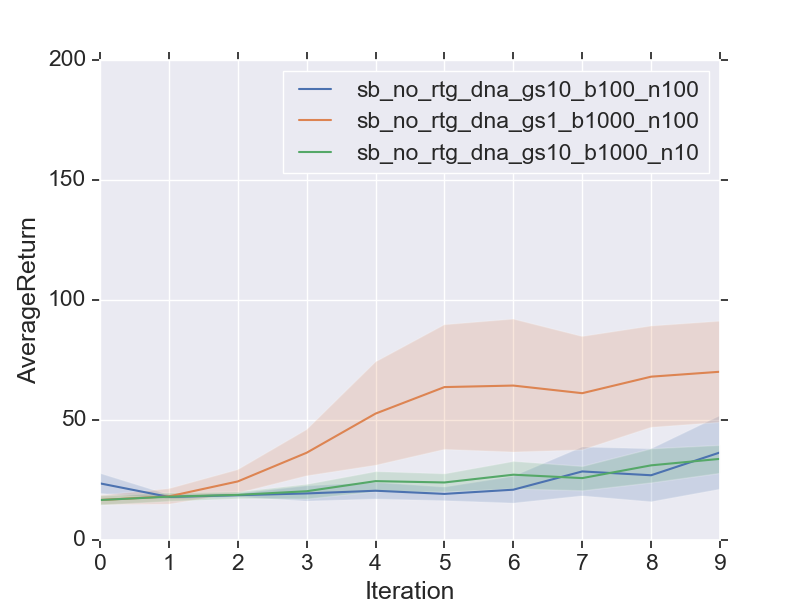
\includegraphics[width=0.5\textwidth]{bonus.png}
	\end{figure}
	\itshape
	\normalfont
	I chose the first environment CartPole-v0 for testing because it's fast. We can see that running multiple gradient steps hurts because policy gradient is a on policy algorithm.
	
	\begin{minipage}{\linewidth}
	\begin{lstlisting}
	# Bonus:
	
	python train_pg_f18.py CartPole-v0 -n 100 -b 100 -e 3 -dna -gs 10 --exp_name sb_no_rtg_dna_gs10_b100_n100
	python train_pg_f18.py CartPole-v0 -n 100 -b 1000 -e 3 -dna -gs 1 --exp_name sb_no_rtg_dna_gs1_b1000_n100
	python train_pg_f18.py CartPole-v0 -n 10 -b 1000 -e 3 -dna -gs 10 --exp_name sb_no_rtg_dna_gs10_b1000_n10
	
	python plot.py data\sb_no_rtg_dna_gs10_b100_n100_CartPole-v0_18-09-2018_09-36-13 data\sb_no_rtg_dna_gs1_b1000_n100_CartPole-v0_18-09-2018_09-43-13 data\sb_no_rtg_dna_gs10_b1000_n10_CartPole-v0_18-09-2018_09-37-17
	\end{lstlisting}
	\end{minipage}
	
\end{document}